\chapter{Parameter Optimization Results}\label{app:optimization results}

\begin{longtable}{l
*{15}{>{\centering\arraybackslash}p{0.6cm}}
}
\caption{Algorithm parameter configurations used in the experiments.}
\label{tab:parameter_configuration}\\
\toprule
\adjustbox{angle=90}{\textbf{Parameter}} &
\adjustbox{angle=90}{\textbf{PSO}} &
\adjustbox{angle=90}{\textbf{PerturbationPSO}} &
\adjustbox{angle=90}{\textbf{RebelPSO}} &
\adjustbox{angle=90}{\textbf{RejectorPSO}} &
\adjustbox{angle=90}{\textbf{RebelRejectorPSO}} &
\adjustbox{angle=90}{\textbf{ContrarianPSO}} &
\adjustbox{angle=90}{\textbf{DefeatistPSO}} &
\adjustbox{angle=90}{\textbf{ContrarianDefeatistPSO}} &
\adjustbox{angle=90}{\textbf{EschewerPSO}} &
\adjustbox{angle=90}{\textbf{EscapistPSO}} &
\adjustbox{angle=90}{\textbf{EschewerEscapistPSO}} &
\adjustbox{angle=90}{\textbf{HybridFullDisjointPSO}} &
\adjustbox{angle=90}{\textbf{HybridPartialDisjointPSO}} &
\adjustbox{angle=90}{\textbf{HybridAdditivePSO}} \\
\midrule
\endfirsthead

\toprule
\adjustbox{angle=90}{\textbf{Parameter}} &
\adjustbox{angle=90}{\textbf{PSO}} &
\adjustbox{angle=90}{\textbf{PerturbationPSO}} &
\adjustbox{angle=90}{\textbf{RebelPSO}} &
\adjustbox{angle=90}{\textbf{RejectorPSO}} &
\adjustbox{angle=90}{\textbf{RebelRejectorPSO}} &
\adjustbox{angle=90}{\textbf{ContrarianPSO}} &
\adjustbox{angle=90}{\textbf{DefeatistPSO}} &
\adjustbox{angle=90}{\textbf{ContrarianDefeatistPSO}} &
\adjustbox{angle=90}{\textbf{EschewerPSO}} &
\adjustbox{angle=90}{\textbf{EscapistPSO}} &
\adjustbox{angle=90}{\textbf{EschewerEscapistPSO}} &
\adjustbox{angle=90}{\textbf{HybridFullDisjointPSO}} &
\adjustbox{angle=90}{\textbf{HybridPartialDisjointPSO}} &
\adjustbox{angle=90}{\textbf{HybridAdditivePSO}} \\
\midrule
\endhead
$N$   & 100 & 100 & 100 & 100 & 100 & 100 & 100 & 100 & 100 & 100 & 100 & 100 & 100 & 100 \\
$\omega$   & 0.063 & 0.637 & 0.131 & 0.084 & 0.116 & 0.102 & 0.069 & 0.067 & 0.091 & 0.047 & 0.088 & 0.010 & 0.054 & 0.043 \\
$c_1$      & 4.373 & 2.545 & 0.308 & 1.545 & 1.292 & 0.405 & 0.405 & 0.905 & 2.177 & 2.577 & 0.900 & 2.519 & 5.251 & 0.254 \\
$c_2$      & 2.755 & 0.789 & 5.531 & 5.918 & 4.833 & 5.729 & 5.296 & 5.063 & 3.649 & 5.865 & 5.271 & 1.959 & 1.044 & 2.307 \\
$c_3$      & --    & --    & 3.923 & --    & 3.745 & --    & --    & --    & --    & --    & --    & 1.523 & 0.445 & 0.041 \\
$c_4$      & --    & --    & --    & 0.466 & 1.441 & --    & --    & --    & --    & --    & --    & 0.805 & 0.108 & 1.304 \\
$c_5$      & --    & --    & --    & --    & --    & 4.560 & --    & 4.333 & --    & --    & --    & 4.525 & 0.792 & 2.243 \\
$c_6$      & --    & --    & --    & --    & --    & --    & 0.953 & 1.746 & --    & --    & --    & 0.353 & 0.068 & 0.137 \\
$c_7$      & --    & --    & --    & --    & --    & --    & --    & --    & 1.658 & --    & 4.853 & 3.545 & 3.732 & 2.769 \\
$c_8$      & --    & --    & --    & --    & --    & --    & --    & --    & --    & 0.059 & 1.582 & 2.257 & 5.558 & 0.023 \\
$\sigma$   & --    & 0.008 & --    & --    & --    & --    & --    & --    & --    & --    & --    & --    & --    & --    \\
$\rho_1$   & --    & --    & --    & --    & --    & --    & --    & --    & --    & --    & --    & --    & --    & 0.880 \\
$\rho_2$   & --    & --    & --    & --    & --    & --    & --    & --    & --    & --    & --    & --    & --    & 0.764 \\
$\rho_3$   & --    & --    & 0.180 & --    & 0.189 & --    & --    & --    & --    & --    & --    & 0.071 & 0.114 & 0.476 \\
$\rho_4$   & --    & --    & --    & 0.679 & 0.194 & --    & --    & --    & --    & --    & --    & 0.353 & 0.393 & 0.536 \\
$\rho_5$   & --    & --    & --    & --    & --    & 0.480 & --    & 0.122 & --    & --    & --    & 0.035 & 0.365 & 0.460 \\
$\rho_6$   & --    & --    & --    & --    & --    & --    & 0.528 & 0.192 & --    & --    & --    & 0.388 & 0.570 & 0.539 \\
$\rho_7$   & --    & --    & --    & --    & --    & --    & --    & --    & 0.224 & --    & 0.163 & 0.136 & 0.172 & 0.315 \\
$\rho_8$   & --    & --    & --    & --    & --    & --    & --    & --    & --    & 0.476 & 0.230 & 0.016 & 0.038 & 0.463 \\
\bottomrule
\end{longtable}


\begin{figure}[H]
    \centering
    \begin{subfigure}{0.49\textwidth}
        \centering
        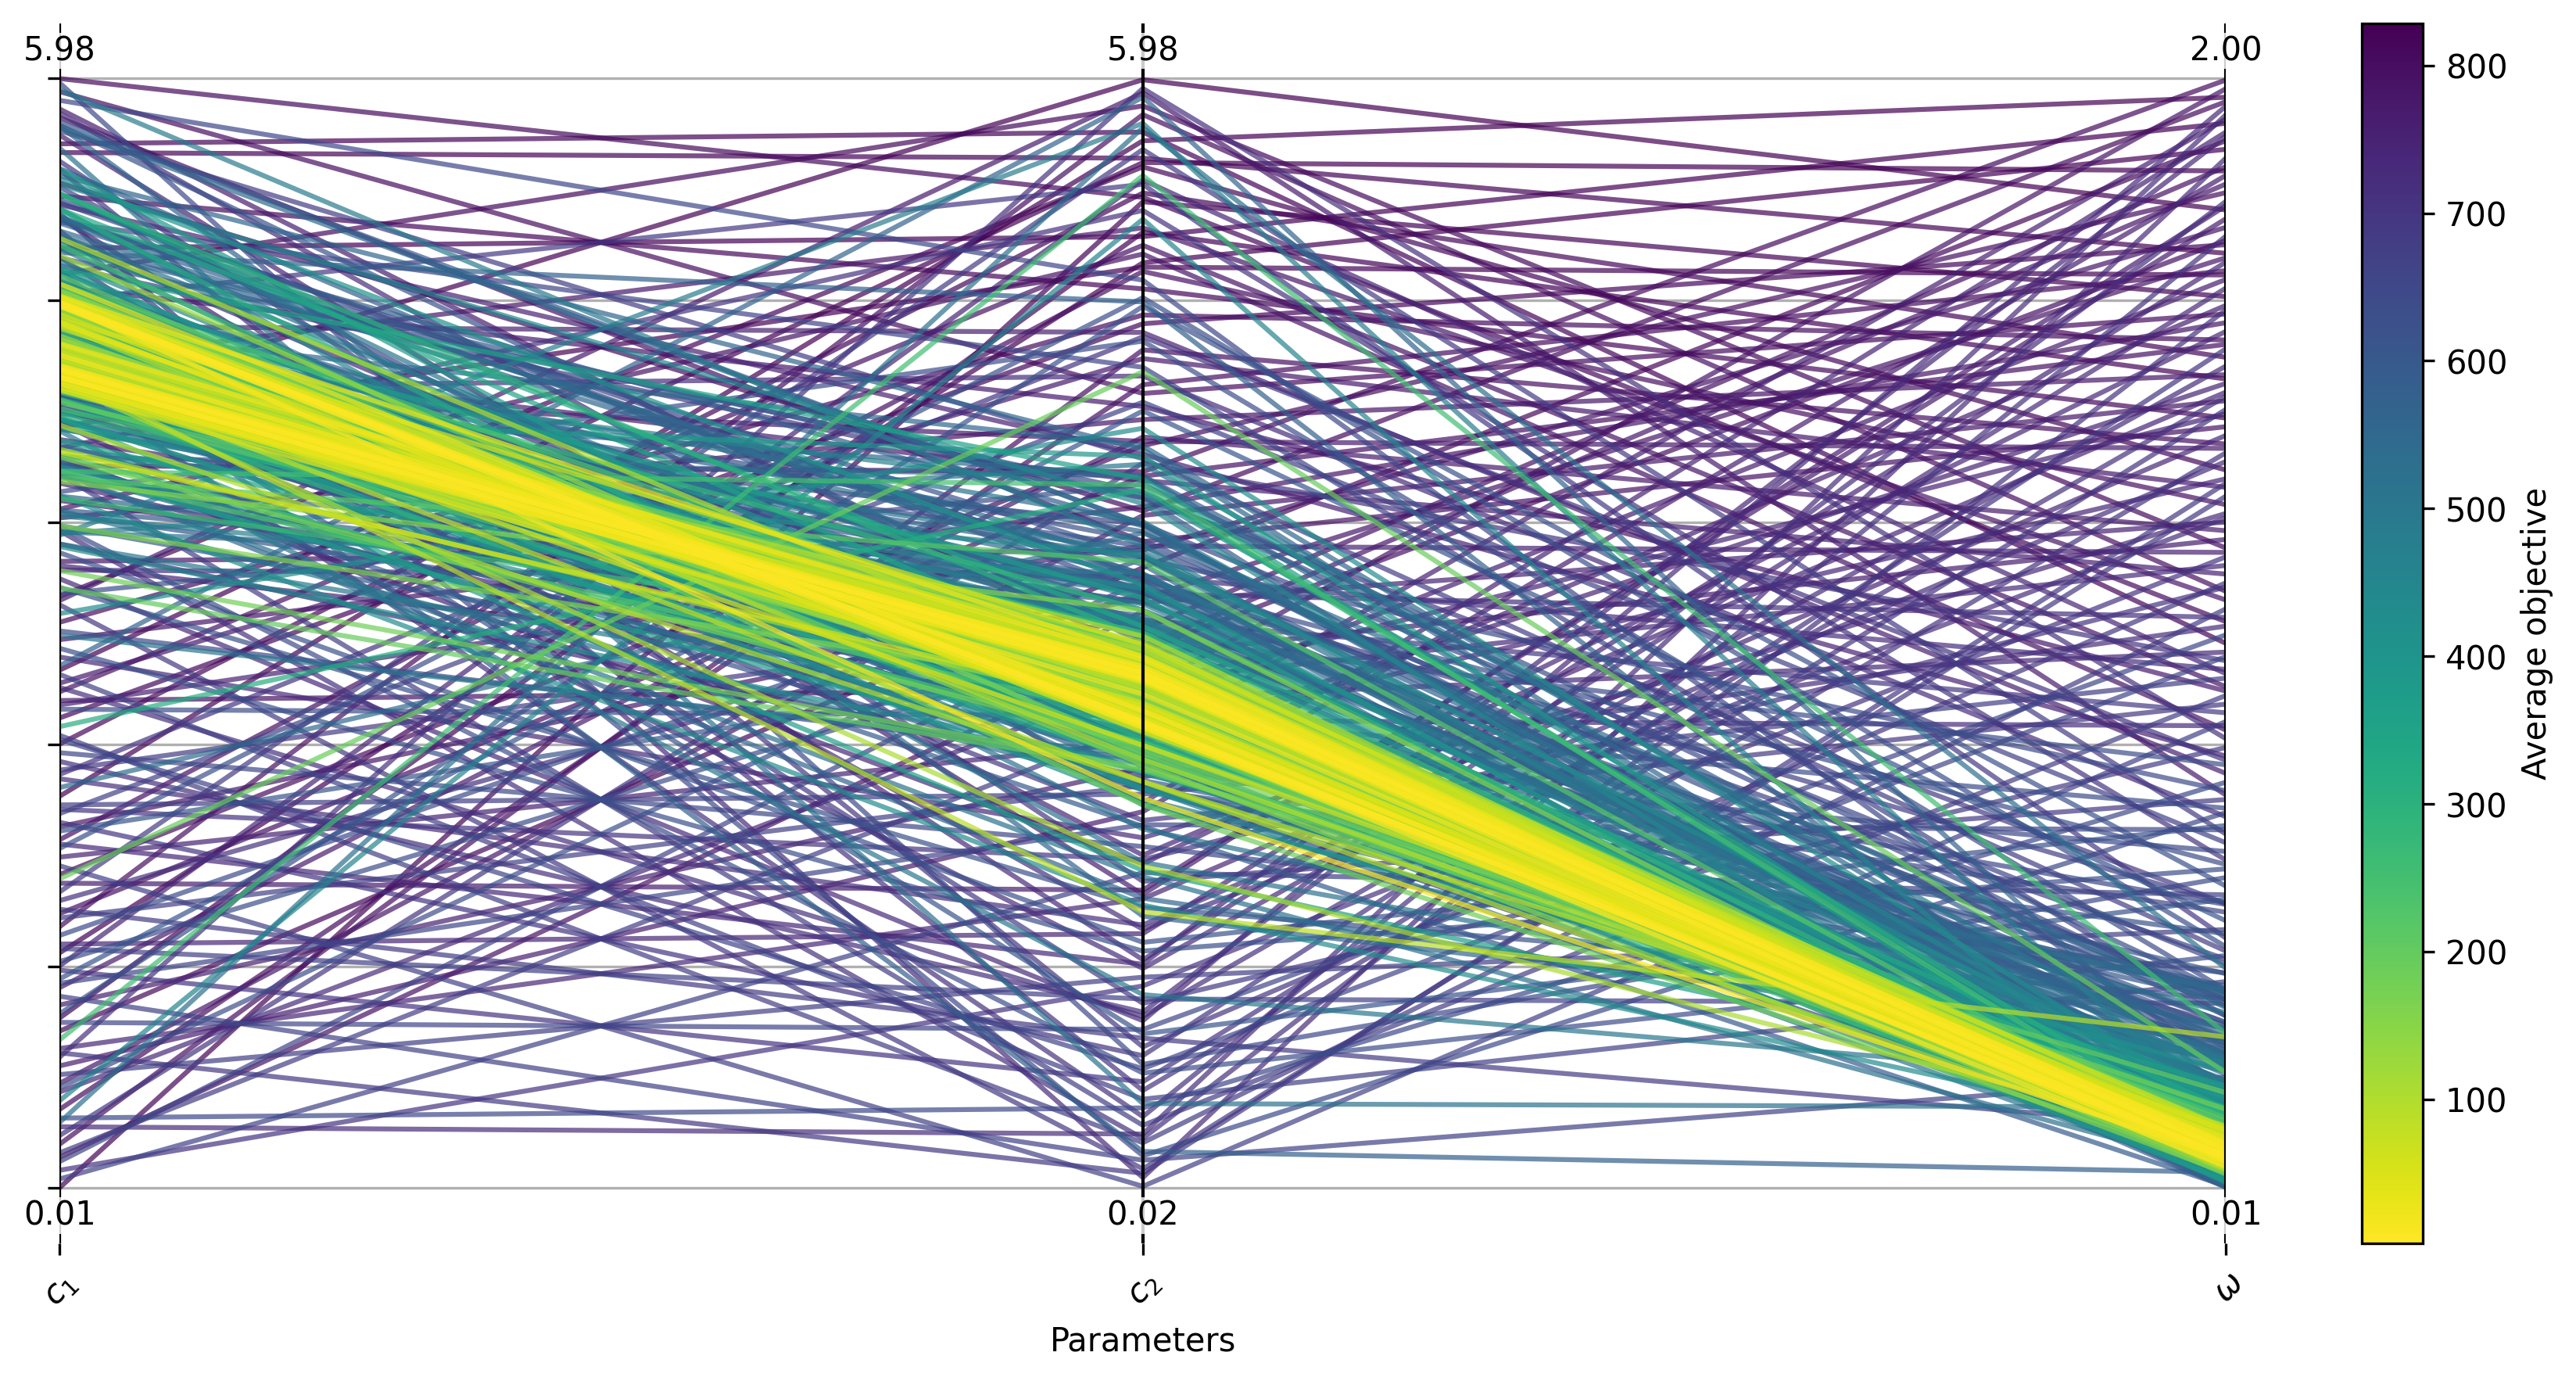
\includegraphics[width=1\textwidth]{Figures/tuning_plots/Parallel_coordinates_plot_for_PSO_parameters.png}
        \caption{PSO}
    \end{subfigure}
    % \hspace{.5cm} % Adjust the space as needed.
    \begin{subfigure}{0.49\textwidth}
        \centering
        \includegraphics[width=1\textwidth]{Figures/tuning_plots/Parallel_coordinates_plot_for_PerturbationPSO_parameters.png}
        \caption{PerturbationPSO}
    \end{subfigure}
    \begin{subfigure}{0.49\textwidth}
        \centering
        \includegraphics[width=1\textwidth]{Figures/tuning_plots/Parallel_coordinates_plot_for_RebelPSO_parameters.png}
        \caption{RebelPSO}
    \end{subfigure}
    % \hspace{.5cm} % Adjust the space as needed.
    \begin{subfigure}{0.49\textwidth}
        \centering
        \includegraphics[width=1\textwidth]{Figures/tuning_plots/Parallel_coordinates_plot_for_RejectorPSO_parameters.png}
        \caption{RejectorPSO}
    \end{subfigure}
        \begin{subfigure}{0.49\textwidth}
        \centering
        \includegraphics[width=1\textwidth]{Figures/tuning_plots/Parallel_coordinates_plot_for_RebelRejectorPSO_parameters.png}
        \caption{RebelRejectorPSO}
    \end{subfigure}
        \begin{subfigure}{0.49\textwidth}
        \centering
        \includegraphics[width=1\textwidth]{Figures/tuning_plots/Parallel_coordinates_plot_for_ContrarianPSO_parameters.png}
        \caption{ContrarianPSO}
    \end{subfigure}
        \begin{subfigure}{0.49\textwidth}
        \centering
        \includegraphics[width=1\textwidth]{Figures/tuning_plots/Parallel_coordinates_plot_for_DefeatistPSO_parameters.png}
        \caption{DefeatistPSO}
    \end{subfigure}
      \begin{subfigure}{0.49\textwidth}
        \centering
        \includegraphics[width=1\textwidth]{Figures/tuning_plots/Parallel_coordinates_plot_for_ContrarianDefeatistPSO_parameters.png}
        \caption{ContrarianDefeatistPSO}
    \end{subfigure}
        \begin{subfigure}{0.49\textwidth}
        \centering
        \includegraphics[width=1\textwidth]{Figures/tuning_plots/Parallel_coordinates_plot_for_EschewerPSO_parameters.png}
        \caption{EschewerPSO}
    \end{subfigure}
    \begin{subfigure}{0.49\textwidth}
        \centering
        \includegraphics[width=1\textwidth]{Figures/tuning_plots/Parallel_coordinates_plot_for_EscapistPSO_parameters.png}
        \caption{EscapistPSO}
    \end{subfigure}
            \captionsetup{list=no}
\caption[Parallel coordinates plots of parameter configurations]{Parallel coordinates plots showing the distribution of  parameter configurations, colored by their average objective value.}
\end{figure}


\begin{figure}[t]\ContinuedFloat
    \centering
    \begin{subfigure}{0.49\textwidth}
        \centering
        \includegraphics[width=1\textwidth]{Figures/tuning_plots/Parallel_coordinates_plot_for_EschewerEscapistPSO_parameters.png}
        \caption{EschewerEscapistPSO}
    \end{subfigure}
    % \hspace{.5cm} % Adjust the space as needed.
    \begin{subfigure}{0.49\textwidth}
        \centering
        \includegraphics[width=1\textwidth]{Figures/tuning_plots/Parallel_coordinates_plot_for_HybridFullDisjointPSO_parameters.png}
        \caption{HybridFullDisjointPSO}
    \end{subfigure}
    \begin{subfigure}{0.49\textwidth}
        \centering
        \includegraphics[width=1\textwidth]{Figures/tuning_plots/Parallel_coordinates_plot_for_HybridPartialDisjointPSO_parameters.png}
        \caption{HybridPartialDisjointPSO}
    \end{subfigure}
    % \hspace{.5cm} % Adjust the space as needed.
    \begin{subfigure}{0.49\textwidth}
        \centering
        \includegraphics[width=1\textwidth]{Figures/tuning_plots/Parallel_coordinates_plot_for_HybridAdditivePSO_parameters.png}
        \caption{HybridAdditivePSO}
    \end{subfigure}
\caption[Parallel coordinates plots of parameter configurations]{Parallel coordinates plots showing the distribution of  parameter configurations, colored by their average objective value.}
\label{fig:parameter_plots}
\end{figure}